\documentclass[reprint,english,notitlepage]{revtex4-1}  % 

\usepackage{silence}
\WarningFilter{revtex4-1}{Repair the float}

\usepackage[utf8]{inputenc}
\usepackage[english]{babel}
\usepackage{physics,amssymb} 
\usepackage{graphicx}        
\usepackage{xcolor}          
\usepackage{hyperref}        
\usepackage{tikz}             
\usepackage{listings} 
\usepackage{csquotes}
\usepackage{subfigure}  
\usepackage{here}
\usepackage{fontawesome}
\bibliographystyle{plain}
\hypersetup{ % this is just my personal choice, feel free to change things
    colorlinks,
    linkcolor={red!50!black},
    citecolor={blue!50!black},
    urlcolor={blue!80!black}}

%% Defines the style of the programming listing
%% This is actually my personal template, go ahead and change stuff if you want
\lstset{ %
	inputpath=,
	backgroundcolor=\color{white!88!black},
	basicstyle={\ttfamily\scriptsize},
	commentstyle=\color{magenta},
	language=Python,
	morekeywords={True,False},
	tabsize=4,
	stringstyle=\color{green!55!black},
	frame=single,
	keywordstyle=\color{blue},
	showstringspaces=false,
	columns=fullflexible,
	keepspaces=true}

%% TiKz stuff
\usetikzlibrary{positioning,chains}
\colorlet{myred}{red!80!black}
\colorlet{myblue}{blue!80!black}
\colorlet{mygreen}{green!60!black}
\colorlet{myorange}{orange!70!red!60!black}
\colorlet{mydarkred}{red!30!black}
\colorlet{mydarkblue}{blue!40!black}
\colorlet{mydarkgreen}{green!30!black}

\definecolor{mako1}{HTML}{38aaac}
\definecolor{mako2}{HTML}{357ba3}
\definecolor{mako3}{HTML}{40498e}


\begin{document}

%==========================================================
%------------------ Project content -----------------------
%==========================================================

%------------------ Abstract ------------------------------
% %================================================================
%------------------------- Abstract -----------------------------
%================================================================
% You summarize your work short and sweet, and reveal very sensible findings. Good! For an abstract, it is customary to include some stage setting at the beginning. The first sentence should reveal what field we are in. The next few might narrow in on which specific subfield we are in. Then, you explain your motivation, or present the "gap" in knowledge that your research will fill.

% Of course, it's not easy to make a motivation for this project, because it is just a project! But I encourage you to attempt to create a motivation that corresponds to the results you want to highlight here. For example, maybe you see a need to explore when to use OLS versus Ridge, because OLS performs better than Ridge unless there's overfitting. It's up to you :) 


% The abstract can then conclude with the broader impact of your findings. What does it mean for the scientific community? Or the general public?
\begin{abstract}
    In this project, I have studied three regression methods, Ordinary Least Squares (OLS), Ridge and Lasso, and compared their performance on synthetic and real terrain data. I found that the choice of method relies on the problem to be solved, and that the OLS method is sufficient when using noise free synthetic data from the Franke function. When introducing noise to the function, Ridge regression performed better as it did not overfit the data. I also performed a bias-variance trade-off analysis, using resampling methods such as bootstrap and cross-validation, and found the optimal polynomial degree for the input data.
\end{abstract}

%------------------ Content overview ----------------------
% \frontmatter      % Folios in Roman numerals
% \tableofcontents  

%------------------ Title ---------------------------------
% \input{sections/titlepage}
\title{Title}
\author{Janita Ovidie Sandtrøen Willumsen \\ \faGithub \, \url{https://github.com/jovidie/FYS-STK4155}}        
\date{\today}
\noaffiliation

% %================================================================
%------------------------- Abstract -----------------------------
%================================================================
% You summarize your work short and sweet, and reveal very sensible findings. Good! For an abstract, it is customary to include some stage setting at the beginning. The first sentence should reveal what field we are in. The next few might narrow in on which specific subfield we are in. Then, you explain your motivation, or present the "gap" in knowledge that your research will fill.

% Of course, it's not easy to make a motivation for this project, because it is just a project! But I encourage you to attempt to create a motivation that corresponds to the results you want to highlight here. For example, maybe you see a need to explore when to use OLS versus Ridge, because OLS performs better than Ridge unless there's overfitting. It's up to you :) 


% The abstract can then conclude with the broader impact of your findings. What does it mean for the scientific community? Or the general public?
\begin{abstract}
    In this project, I have studied three regression methods, Ordinary Least Squares (OLS), Ridge and Lasso, and compared their performance on synthetic and real terrain data. I found that the choice of method relies on the problem to be solved, and that the OLS method is sufficient when using noise free synthetic data from the Franke function. When introducing noise to the function, Ridge regression performed better as it did not overfit the data. I also performed a bias-variance trade-off analysis, using resampling methods such as bootstrap and cross-validation, and found the optimal polynomial degree for the input data.
\end{abstract}
\maketitle

%------------------ Body ----------------------------------
% \mainmatter
% Scaling: the franke function uses samples from 0 to 1, careful with scaling as the $x^{p-1}$ would end up close to zero. 
% %================================================================
\section{Introduction}\label{sec:introduction}
% Motivate the reader and present overarching ideas, and 
% background on the subject of the project. Mention what I have 
% done and present the structure of the report, that is how it is 
% organized.
%================================================================
- Machine learning intro
- ML specific to this problem
- Report structure
% \input{project-1/sections/theory}
%================================================================
\section{Methods}\label{sec:methods}
% Describe the methods and algorithms used, include any formulas. 
% Explain how everything is implemented, and possibly mention the 
% structure of the algorithm. Add demonstrations such as tests, 
%  selected runs and validations. 
%================================================================

\subsection{Data}\label{ssec:data}
To train the model we need data which resemble our problem. The Franke function \eqref{eq:franke_function} is used as a test function in problems dealing with interpolation, and will be used to generate dataset. 

\begin{equation}\label{eq:franke_function}
\begin{split}
    f(x, y) &= \frac{3}{4} \exp(- \frac{(9x-2)^{2}}{4} - \frac{(9y-2)^{2}}{4} ) \\
    &+ \frac{3}{4} \exp(- \frac{(9x-2)^{2}}{4} - \frac{(9y-2)^{2}}{4} ) \\
    &+ \frac{3}{4} \exp(- \frac{(9x+1)^{2}}{49} - \frac{(9y+1)}{10} ) \\ 
    &- \frac{1}{5} \exp(- (9x-4)^{2} - (9y-7)^{2} ) 
\end{split}
\end{equation}
- Topographic data
- Preprocessing


\subsection{Regression models}\label{ssec:regression_models}
- OLS
- Ridge
- Lasso

\subsection{Resampling techniques}\label{ssec:resampling_techniques}
- Bootstrap
- Cross-validation

\subsection{Model evaluation}\label{ssec:evaluation}
- Bias-variance trade off


\subsection{Tools}\label{ssec:tools}
% %================================================================
\section{Results}\label{sec:results}
% Present results and give a critical discussion of my work in 
% the context of other work. Relate the work to previous studies, 
% and make sure the results are reproducible. Include information 
% in figure captions such that they can give the reader enough to 
% understand the main gist of the report.
%================================================================
\subsection{Synthetic data analysis}\label{ssec:synthetic_data}
I generated two synthetic data set, one of which included stochastic noise, from the Franke function in Equation \eqref{eq:franke_function}. To keep the initial analysis efficient and interpretable, I used $50 \times 50$ data points and noise $\epsilon \sim \mathcal{N}(0, 0.1)$. 

\subsubsection{Ordinary Least Squares}\label{sssec:ols_synthetic}
I performed an OLS regression analysis up to a fifth polynomial degree, and computed the MSE and R$^{2}$-score for performance on both data set. The model's coefficients are shown in Figure \ref{fig:ols_beta_smooth} and Figure \ref{fig:ols_beta}. The MSE and R$^{2}$-score is shown in Figure \ref{fig:ols_error_smooth} and Figure \ref{fig:ols_error}.
\begin{figure}[h]
    \centering
    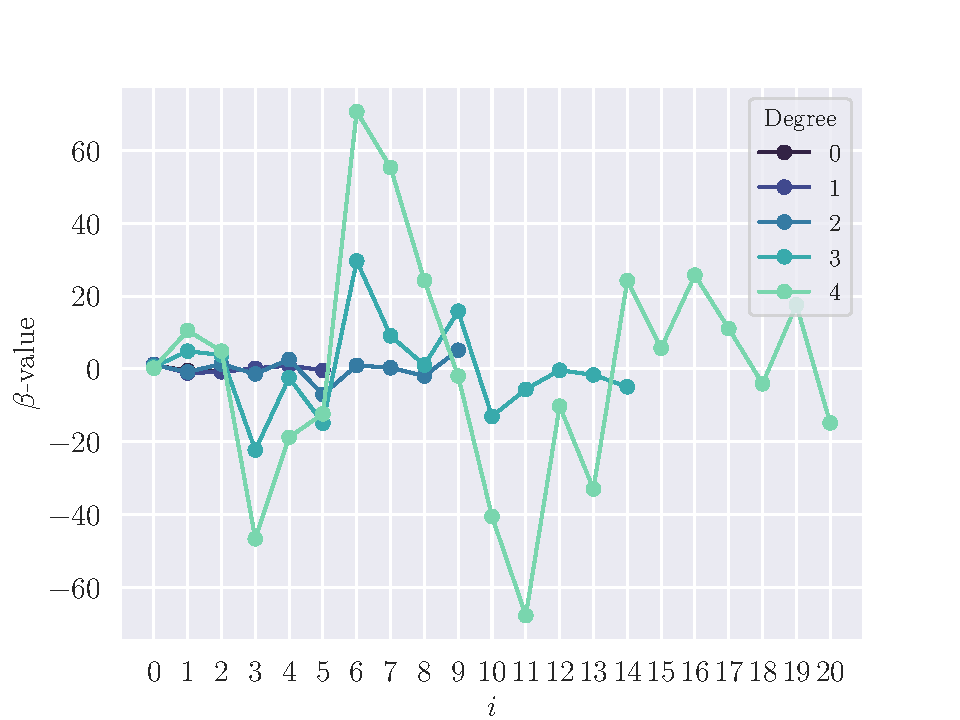
\includegraphics[width=\linewidth]{project-1/latex/figures/ols_beta_smooth_N50.pdf}
    \caption{The figure shows $\beta$ values for the OLS model, with features of polynomial degree up to fifth order. The index $i$ denotes the index of $\beta_{i}$.The model was trained and tested on synthetic data without stochastic noise.}
    \label{fig:ols_beta_smooth}
\end{figure}
\begin{figure}[h]
    \centering
    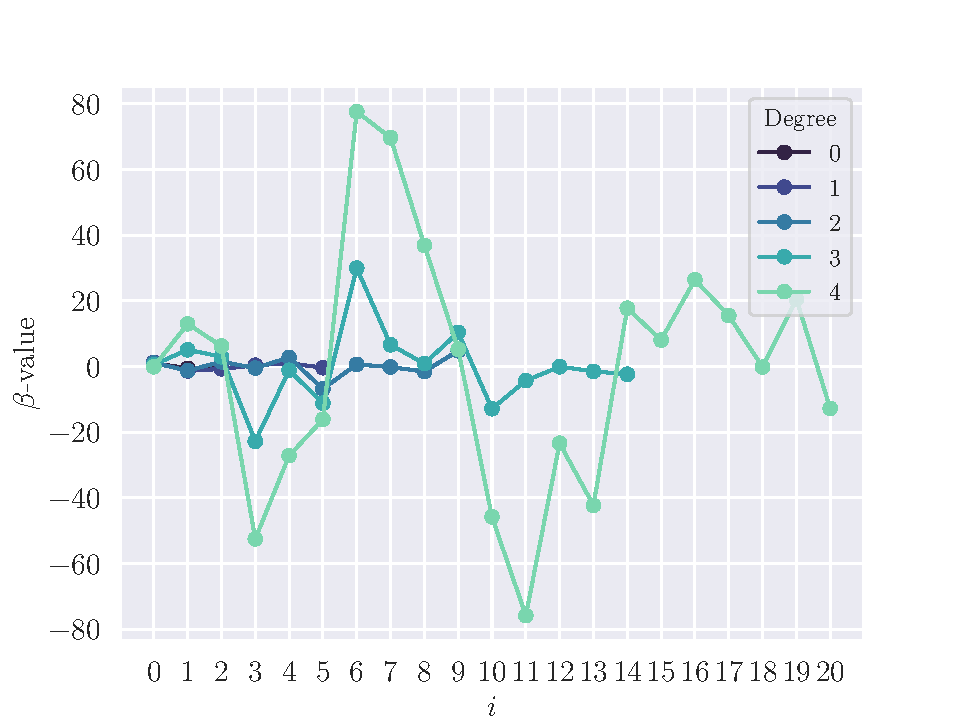
\includegraphics[width=\linewidth]{project-1/latex/figures/ols_beta_N50.pdf}
    \caption{The figure shows $\beta$ values for the OLS model, with features of polynomial degree up to fifth order. The index $i$ denotes the index of $\beta_{i}$. The model was trained and tested on synthetic data which included stochastic noise $\mathcal{N}(0, 0.1)$.}
    \label{fig:ols_beta}
\end{figure}
\begin{figure}[h]
    \centering
    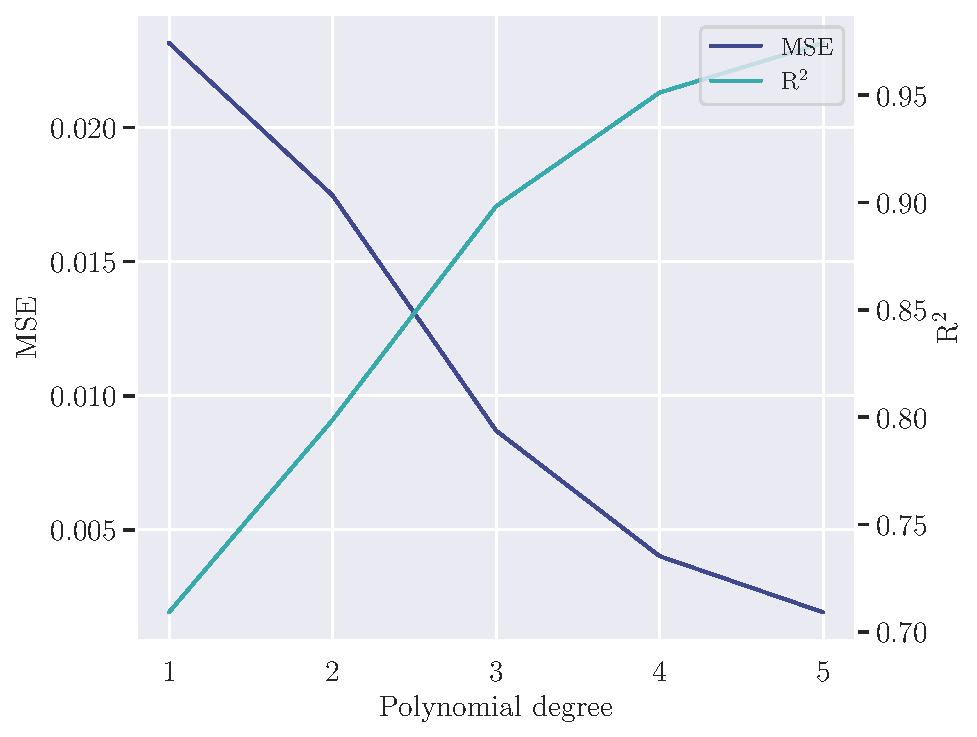
\includegraphics[width=\linewidth]{project-1/latex/figures/ols_error_smooth_N50.pdf}
    \caption{MSE and R$^{2}$-score computed from OLS' performance on test data, as a function of the polynomial degree of the input features. The model was trained and tested on synthetic data without stochastic noise.}
    \label{fig:ols_error_smooth}
\end{figure}
\begin{figure}[h]
    \centering
    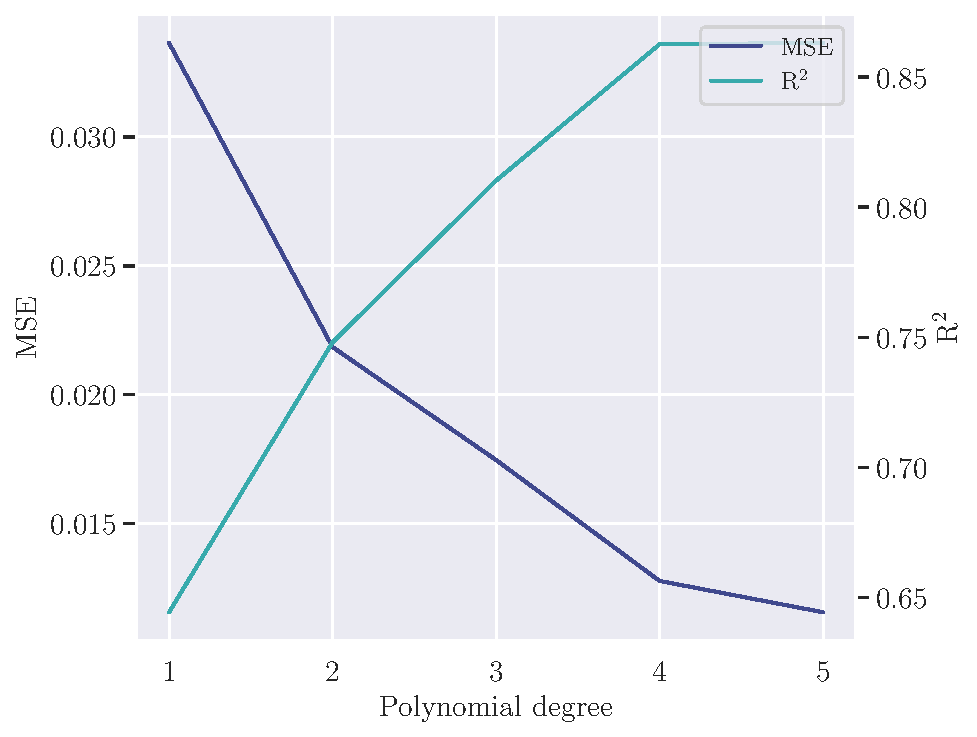
\includegraphics[width=\linewidth]{project-1/latex/figures/ols_error_N50.pdf}
    \caption{MSE and R$^{2}$-score computed from OLS' performance on test data, as a function of the polynomial degree of the input features. The model was trained and tested on synthetic data which included stochastic noise $\mathcal{N}(0, 0.1)$.}
    \label{fig:ols_error}
\end{figure}
In addition, I performed the analysis with feature scaling, the resulting figures can be found in \ref{ap:additional_analysis}.

When increasing the order of polynomial features, the coefficient $\beta$ increase in value as well as variance. The error decrease with the increase of polynomial order, suggesting the model is better able to explain the complexity of the data. Which is confirmed by comparing the result in Figure \ref{fig:ols_error_smooth} and Figure \ref{fig:ols_error}, the model performs better on data which does not include noise.
%------------ Hastie -----------------------------
I continued with the OLS model, and synthetic data which included noise. To study the model performance on both the training data and test data, as the order of the polynomial degree was increased to $18$. The result is shown in Figure \ref{fig:ols_hastie}.
\begin{figure}[h]
    \centering
    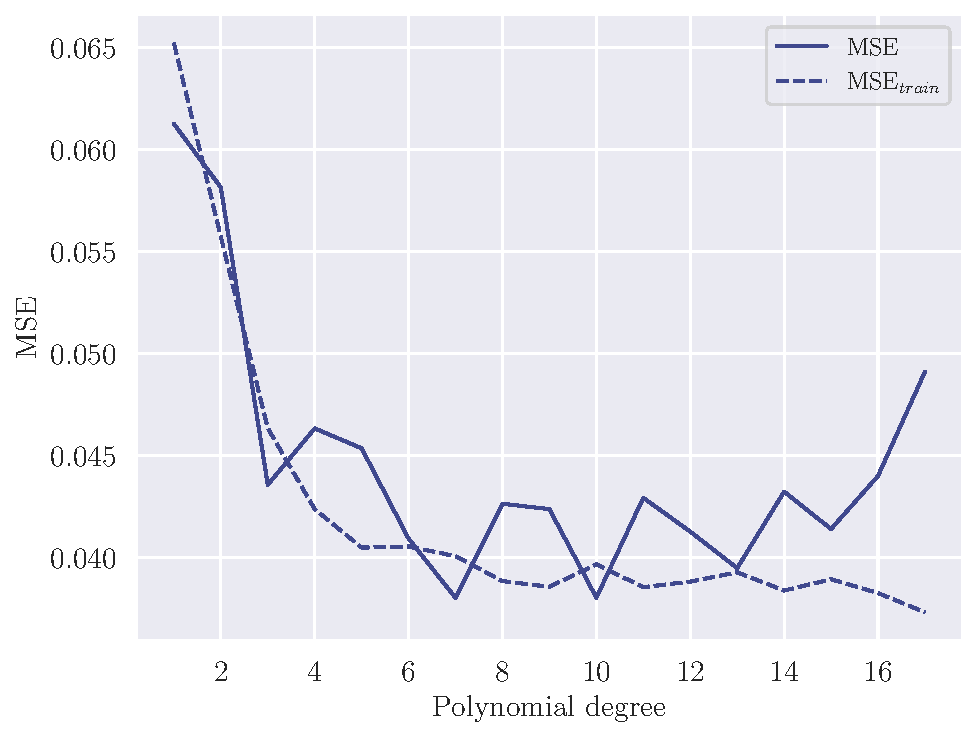
\includegraphics[width=\linewidth]{project-1/latex/figures/dev-figs/ols_hastie_N50.pdf}
    \caption{MSE computed from OLS' performance on train and test data, as a function of the polynomial degree of the input features. The data included stochastic noise $\mathcal{N}(0, 0.1)$.}
    \label{fig:ols_hastie}
\end{figure}\ref{ap:additional_analysis}
As the polynomial degree increase, both train and test error decrease. However, around degree $7$ the test error varies and increase, whereas the train error continue to decrease. Since the model is fit to the training data, this trend indicate that the model is overfit to the training data and is not able to generalize to new data. This also suggest that the order of the polynomial degree is higher than what is necessary to explain the data. This result varied with the seed given, here I used seed $12$ as it gave an interpretable figure. For the rest of the project, I used seed $2024$. I will explore the effect of overfitting later, when I study resampling and the bias-variance trade-off. To study the effect of regularization, I continued with the synthetic data which includes noise.


\subsubsection{Ridge}\label{sssec:ridge_synthetic}
To determine a range for the optimal values of $\lambda$, I trained and tested the Ridge model on $100$ values, where Log$_{10}(\lambda) \in [-15, 5]$. The result can be found in Figure \ref{fig:lmbda_opt}, in Appendix \ref{ap:additional_analysis}. The analysis indicated that smaller values were likely better for further analysis. 
\begin{table}[h]
    \centering
    \begin{tabular}{cc}
        \hline
        $\lambda_{i}$ & Value \\
        \hline 
        $\lambda_{1}$ & $1.00e-05$ \\
        $\lambda_{2}$ & $2.68e-05$ \\
        $\lambda_{3}$ & $7.20e-05$ \\
        $\lambda_{4}$ & $1.93e-04$ \\
        $\lambda_{5}$ & $5.18e-04$ \\
        $\lambda_{6}$ & $1.39e-03$ \\
        $\lambda_{7}$ & $3.73e-03$ \\
        $\lambda_{8}$ & $1.00e-02$ \\
        \hline
    \end{tabular}
    \caption{Approximate values of $\lambda$, generated using a logspace function and the range $[-5, -2]$. The values was used in both Ridge and Lasso regression analysis.}
    \label{tab:lambdas}
\end{table}
I continued with $8$ values, found in Table \ref{tab:lambdas}, and performed a Ridge regression analysis up to a $15$ polynomial degree. I computed MSE for performance on the test data, which can be found in Figure \ref{fig:ridge_error}.
\begin{figure}[h]
    \centering
    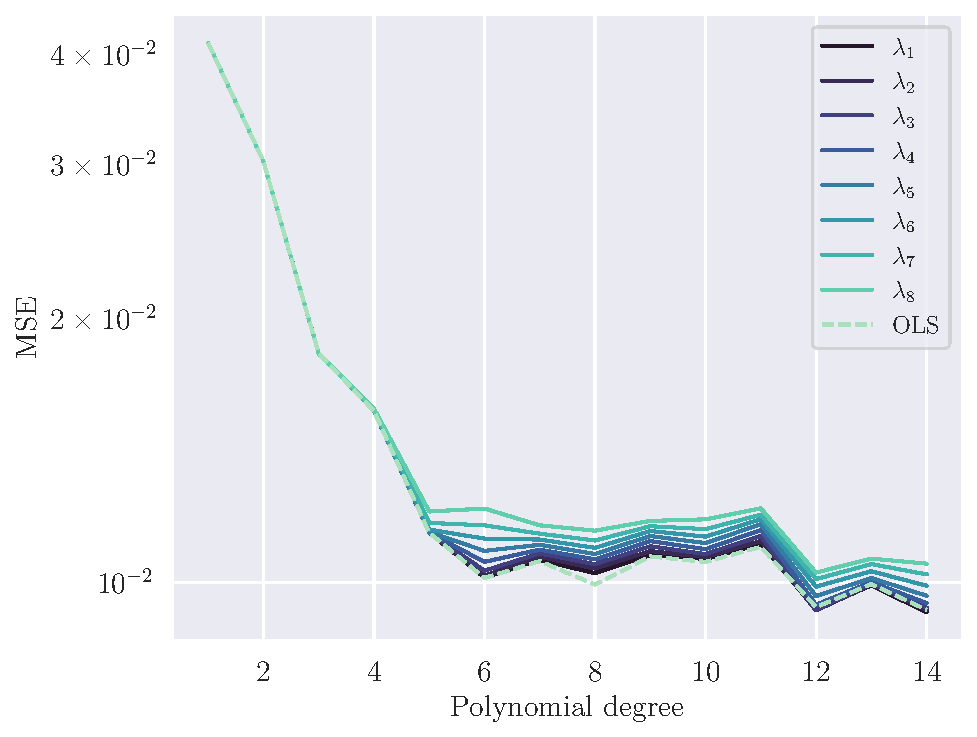
\includegraphics[width=\linewidth]{project-1/latex/figures/ridge_error_scaled_N50.pdf}
    \caption{MSE computed from Ridge regression on test data, as a function of the order of polynomial degree of the input features. The synthetic data included stochastic noise $\mathcal{N}(0, 0.1)$, with standardized feature scaling.}
    \label{fig:ridge_error}
\end{figure}
The MSE decrease for higher order polynomial degree. However, the MSE is larger for larger values of $\lambda$, where $\lambda_{8}$ is the largest value. For OLS, $\lambda$ is technically equal to zero. Ridge regression performs better than OLS for values of $\lambda$ close to zero, when the features are scale. Which is to be expected, since Ridge adds more penalty to larger features. It also performs better on higher order polynomials, as the coefficients are penalized and the model generalizes better. For lower order of complexity, the performance of Ridge regression does not justify the computational cost. 

\subsubsection{Lasso}\label{sssec:lasso_synthetic}
I performed a Lasso regression analysis up to a $15$ polynomial degree, using the values of $\lambda$ found in Table \ref{tab:lambdas}. I computed MSE for performance on the test data, which can be found in Figure \ref{fig:lasso_error}.
\begin{figure}[h]
    \centering
    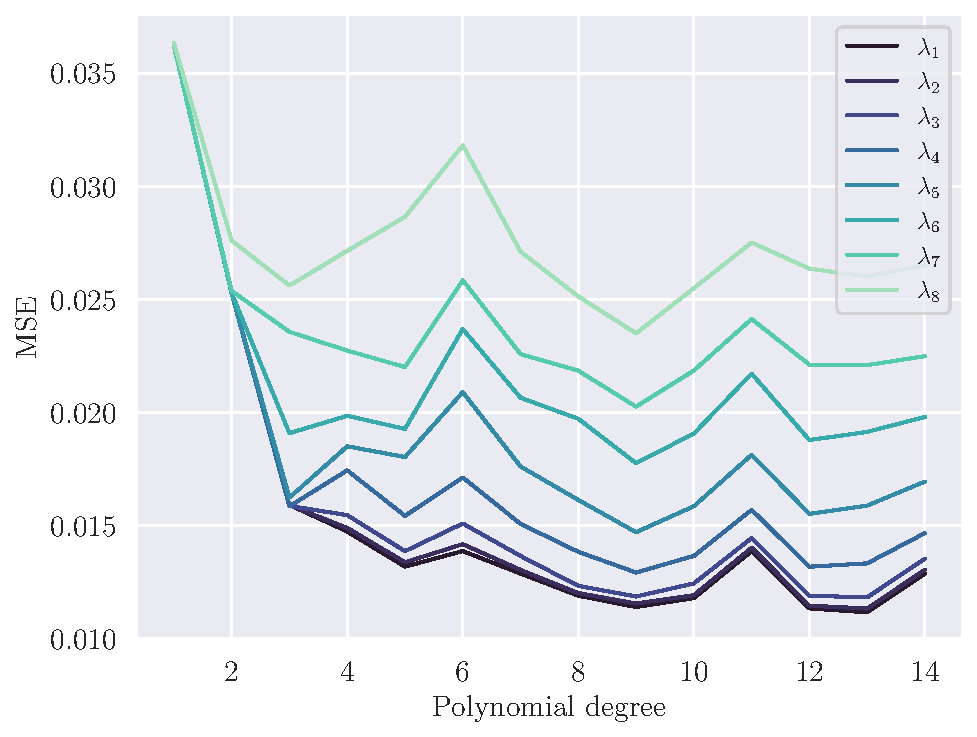
\includegraphics[width=\linewidth]{project-1/latex/figures/lasso_error_scaled_N50.pdf}
    \caption{MSE computed from Lasso regression on test data, as a function of of polynomial order of the input features. The synthetic data included stochastic noise $\mathcal{N}(0, 0.1)$, with standardized feature scaling.}
    \label{fig:lasso_error}
\end{figure}
The Lasso model uses an iterative approach, and tries to converge. However, the model was not able to converge with number of iterations set to $10 000$, and required longer runtime than both OLS and Ridge regression. It also performs as well as OLS for the smallest values of $\lambda$, meaning the performance of Lasso does not justify the computational cost for any order of complexity.

For the synthetic data, the OLS regression model performed best. As the model was able to explain the data complexity as well as, or better than, both Ridge and Lasso regression. For higher order polynomial degree, Ridge regression did have a smaller error, however, in comparison to OLS the gain in performance is not noticeable.

\subsubsection{Bootstrap}\label{sssec:bootstrap_synthetic}
To study the bias-variance trade-off, I performed an OLS regression with bootstrap. The number of bootstraps was set to $100$, with a maximum polynomial degree of $18$. The result is shown in Figure \ref{fig:ols_bootstrap}.
\begin{figure}[h]
    \centering
    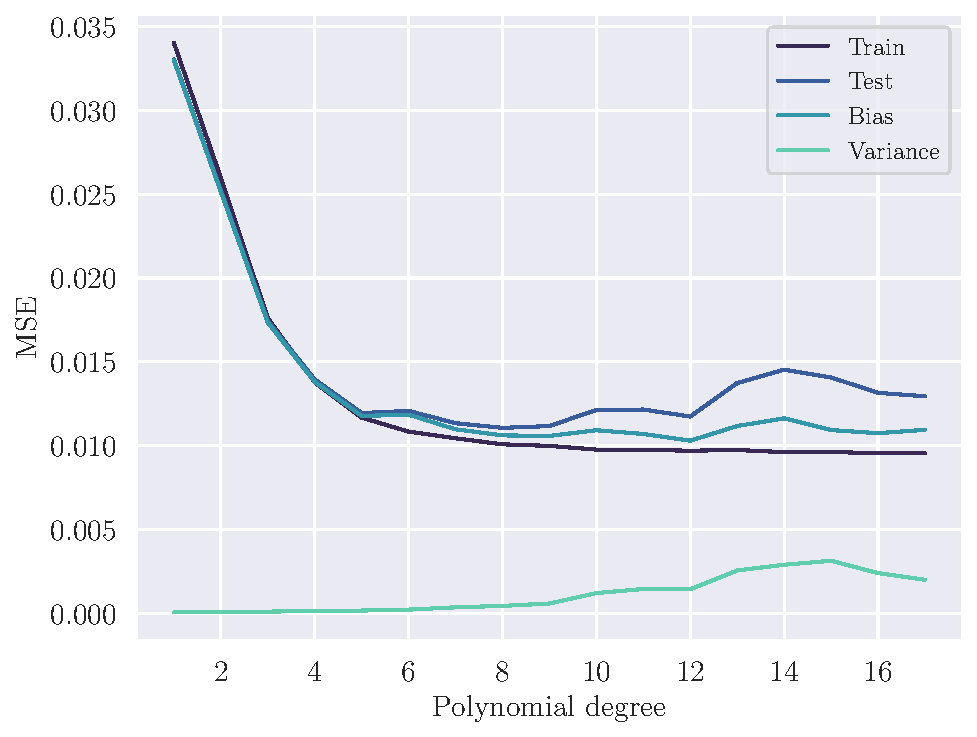
\includegraphics[width=\linewidth]{project-1/latex/figures/ols_bootstrap_100_scaled_N50.pdf}
    \caption{MSE computed from OLS regression, on train and test data, as a function of of polynomial order of the input features. The figure also includes the bias and variance on the test data. The synthetic data included stochastic noise $\mathcal{N}(0, 0.1)$, with standardized feature scaling.}
    \label{fig:ols_bootstrap}
\end{figure}
The train and test error decrease as the polynomial order increase. This is also true for the bias, whereas the variance increase with higher polynomial degree. For this seed, and the low complexity of the data, the trend of bias and variance is not clear. Typically, the bias tend to decrease in the same manner as the train and test error, up to a order of complexity. At this point, the variance increases and crosses the bias, indicating that the model is overfit. A model is good at generalizing to new data, when there is some bias and variance. At this order of complexity, the model is not overfit to the training data, and performs as well on test data.

\subsubsection{Cross-validation}\label{sssec:cross_validation_synthetic}
I continued the analysis evaluating all regression methods using $10$-fold cross-validation, with $\lambda = 1.0e-05$ for Ridge and Lasso regression. The result is shown in Figure \ref{fig:crossval}. I also compared cross-validation with the bootstrap method, which is found in Figure \ref{fig:bootstrap_crossval}.
\begin{figure}[h]
    \centering
    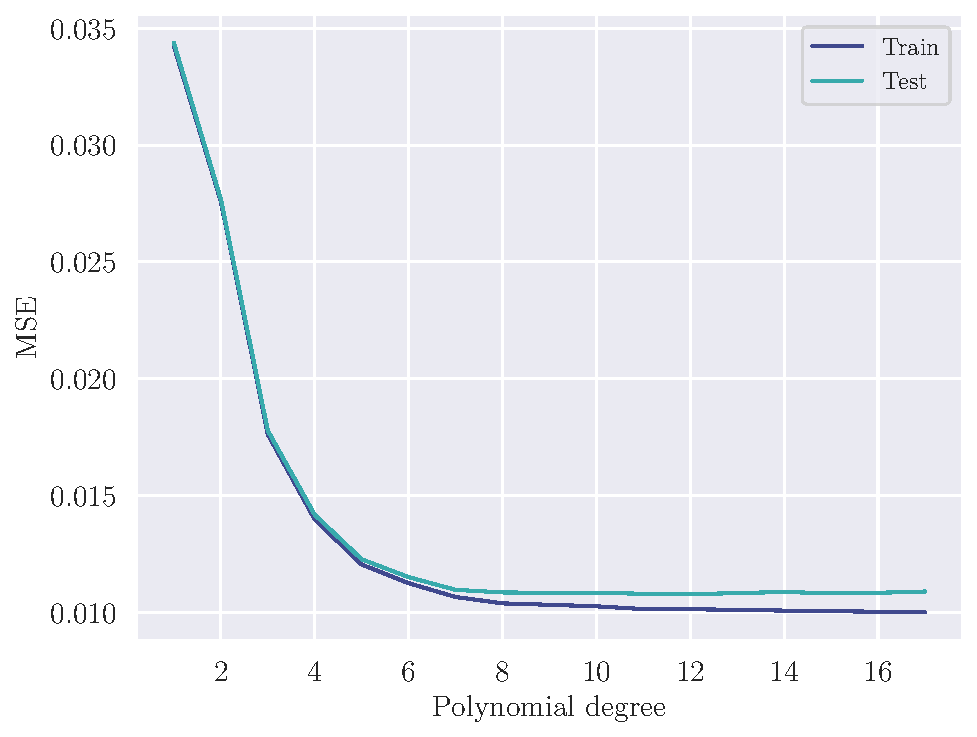
\includegraphics[width=\linewidth]{project-1/latex/figures/ols_crossval_10_N50.pdf}
    \caption{The figure shows MSE of OLS, Ridge, and Lasso regression models, on train (dotted) and test (solid) data, using cross-validation. MSE as a function of of polynomial order of the input features. The synthetic data included stochastic noise $\mathcal{N}(0, 0.1)$, with standardized feature scaling.}
    \label{fig:crossval}
\end{figure}
Cross-validation uses the entire data set in all fit and predict iterations. Meaning some data points might be in the train set in one iteration, and in the test set the next iteration. This result in an optimistic model, as there is data leakage and the model might not be as generalized as the result suggest. One approach to accommodate for the data leakage, is to split the data set in three parts - train, test and validation. This could give a more realistic view of the model performance when new data is introduced. 
\begin{figure}[h]
    \centering
    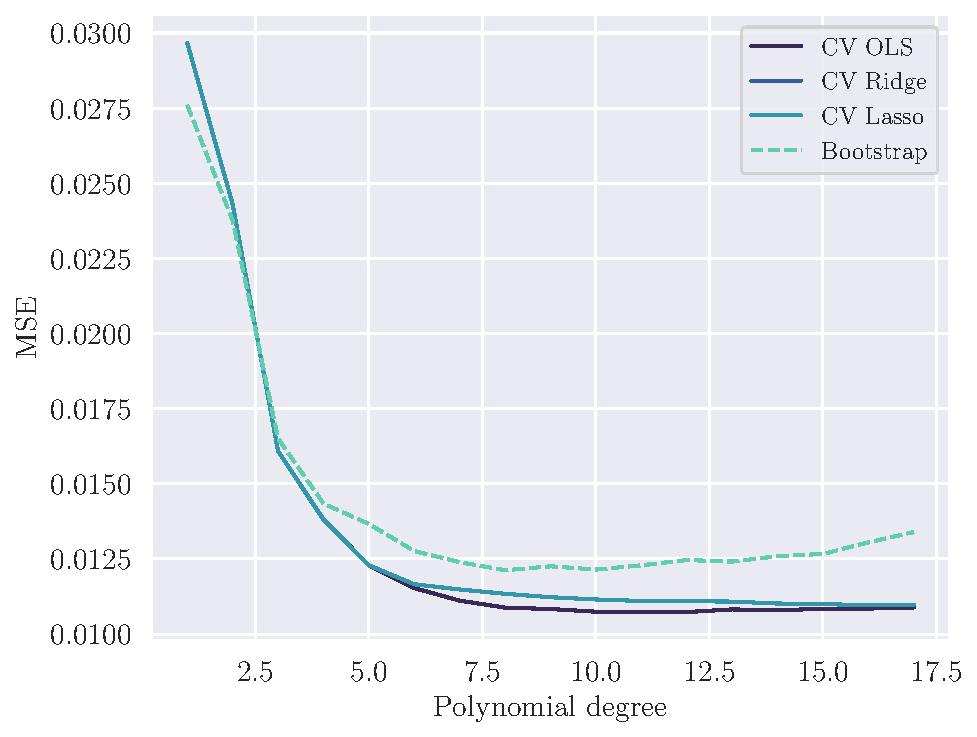
\includegraphics[width=\linewidth]{project-1/latex/figures/ols_bs_crossval_10_N50.pdf}
    \caption{The figure shows MSE of OLS, Ridge, and Lasso regression models, on train (dotted) and test (solid) data, using cross-validation. It also shows MSE for OLS using bootstrap, with $100$ bootstraps. MSE is shown as a function of of polynomial order of the input features. The synthetic data included stochastic noise $\mathcal{N}(0, 0.1)$, with standardized feature scaling.}
    \label{fig:crossval}
\end{figure}
When comparing resampling methods, cross-validation performs better than bootstrap for most polynomial degree. The bootstrap method reach a minimum error at degree $7$, after which the error seem to increase. For lower polynomial degree the OLS regression and bootstrap method is sufficient in capturing the complexity of the data. To study the regression models further, and the effect of data complexity in their performance, I continued the analysis using real terrain data.

\subsection{Terrain data analysis}\label{ssec:terrain_data}
I used satellite data from EarthExplorer, more information on the data can be found in Table \ref{tab:terrain_data} in Appendix \ref{ap:terrain_data}. The following analysis focuses on terrain data from Japan, and the Osaka area. Since the data set is quite large, I used a subset $50 \times 50$, equal to the size of the synthetic data set. In addition, I used feature scaling for all regression methods.

\subsubsection{Ordinary Least Squares}\label{sssec:ols_terrain}
I performed OLS regression on the terrain data, with polynomial features up to degree $15$. The model coefficients for degree $1-5$ is shown in Figure \ref{fig:beta_terrain}, and the computed MSE is shown in Figure \ref{fig:ols_error_terrain}.
\begin{figure}[h]
    \centering
    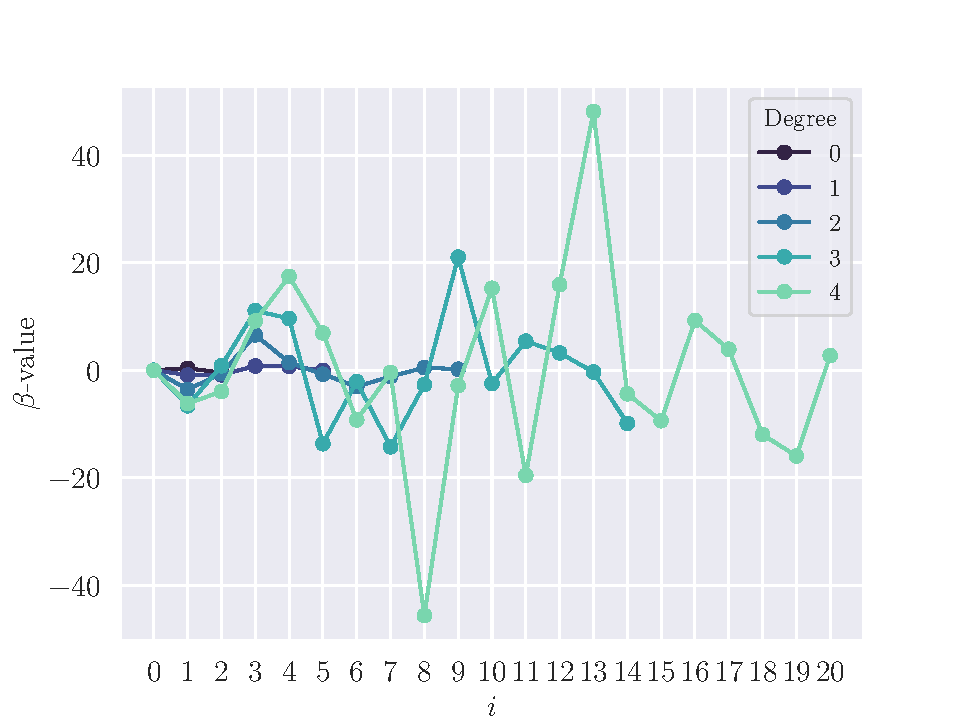
\includegraphics[width=\linewidth]{project-1/latex/figures/ols_beta_terrain_D5_N50.pdf}
    \caption{The figure shows $\beta$ values for the OLS model, with features of polynomial degree up to fifth order. The index $i$ denotes the index of $\beta_{i}$. The model was trained and tested on terrain data, with standardized feature scaling.}
    \label{fig:ols_beta_terrain}
\end{figure}
\begin{figure}[h]
    \centering
    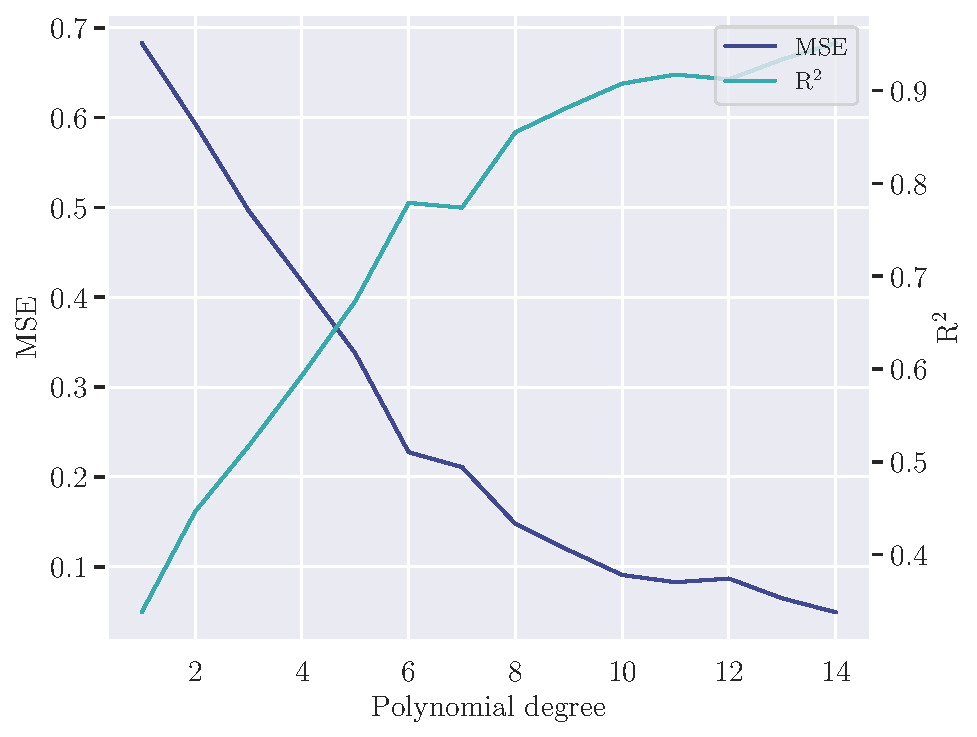
\includegraphics[width=\linewidth]{project-1/latex/figures/ols_error_terrain_N50.pdf}
    \caption{MSE and R$^{2}$-score computed from OLS' performance on test data, as a function of the polynomial degree of the input features. The model was trained and tested on terrain data, with standardized feature scaling.}
    \label{fig:ols_error_terrain}
\end{figure}


\subsubsection{Ridge}\label{sssec:ridge_terrain}


\subsubsection{Lasso}\label{sssec:lasso_terrain}


\subsubsection{Bootstrap}\label{sssec:bootstrap_terrain}


\subsubsection{Cross-validation}\label{sssec:crossval_terrain}
% %================================================================
\section{Conclusion}\label{sec:conclusion}
% State main findings and interpretations, and try to present 
% perspectives for future work. Discuss pros and cons of methodd, 
% and possible improvements.
%================================================================
% Scaling: the franke function uses samples from 0 to 1, careful with scaling as the $x^{p-1}$ would end up close to zero. 
 
%------------------ Bibliography --------------------------
% \newpage 
% \nocite{*}
% \bibliography{references}

%------------------ Appendix ------------------------------
% \newpage
% \onecolumngrid
% \appendix
% %================================================================
\appendix
% Additional calculations used to validate the codes, these 
% selected calculations can be listed with few comments. Can also 
% include listing of the code if you feel this is necessary
%================================================================
\section{Terrain data}\label{ap:terrain_data}
Information on terrain data, downlowdad from EarthExplorer.
\begin{table}[h]
    \centering
    \begin{tabular}{cccc}
        \hline
        Country & ID & Coordinates \\
        \hline
        China & SRTM1N36E110V3 & $(36, 110)$ \\
        Egypt & SRTM1N26E029V3 & $(26, 29)$ \\
        Japan & SRTM1N34E135V3 & $(34, 135)$ \\
        Nepal & SRTM1N27E085V3 & $(27, 85)$ \\
        Norway & SRTM1N59E010V3 & $(59, 10)$ \\
        \hline
    \end{tabular}
    \caption{Terrain data from different countries. The coordinates are with respect to the south west corner of the grid, given in latitude, longitude.}
    \label{tab:terrain_data}
\end{table}


\section{Cost functions}\label{ap:cost_functions}
- OLS
- Ridge
- Lasso


\section{Bias-Variance Trade-Off}\label{ap:bias_var_eq}
The parameters $\mathbf{\beta}$ can be found by optimizing the cost function
\begin{equation*}
    C(\mathbf{X}, \mathbf{\beta}) = \frac{1}{n} \sum_{i=0}^{n-1} ( y_{i} - \Tilde{y}_{i} )^{2} = \mathbb{E} \big[ ( \mathbf{y} - \mathbf{\Tilde{y}} )^{2} \big] .
\end{equation*}

Assuming linearity, the expression can be written as 
\begin{equation*}
    \mathbb{E} \big[ ( \mathbf{y} - \mathbf{\Tilde{y}} )^{2} \big] = \mathbb{E} [ \mathbf{y}^{2} ] - 2 \mathbb{E} [ \mathbf{y} \mathbf{\Tilde{y}} ] + \mathbb{E} [ \mathbf{\Tilde{y}}^{2} ].
\end{equation*}

Looking at the first term
\begin{align*}
    \mathbb{E} [ \mathbf{y}^{2} ] &= \mathbb{E} [ ( f(\mathbf{x}) + \mathbf{\epsilon} )^{2} ] \\
    &= \mathbb{E} [ f(\mathbf{x})^{2} ] - 2 \mathbb{E} [ f(\mathbf{x}) \mathbf{\epsilon} ] + \mathbb{E} [ \mathbf{\epsilon}^{2} ] & \text{where $f(\mathbf{x})$ and $\epsilon$ are independent of $\mathbf{y}$, and each other} \\
    &= f(\mathbf{x})^{2} + \sigma^{2} .
\end{align*}

The second term can be written as 
\begin{align*}
    \mathbb{E} [ \mathbf{y} \mathbf{\Tilde{y}} ] &= \mathbb{E} [ f(\mathbf{x} + \mathbf{\epsilon}) \mathbf{\Tilde{y}} ] \\
    &= \mathbb{E} [ f(\mathbf{x}) \mathbf{\Tilde{y}} ] + \mathbb{E} [ \epsilon \mathbf{\Tilde{y}} ] \\
    &=  f(\mathbf{x}) \mathbb{E} [ \mathbf{\Tilde{y}} ] & \text{since $\mathbb{E}[\mathbf{\epsilon}] = 0$} .
\end{align*}

The last term is the 2. moment, which can be written as 
\begin{align*}
    \mathbb{E} [ \mathbf{\Tilde{y}}^{2} ] &= \mathbb{V}[\mathbf{\Tilde{y}}] + (\mathbb{E} [ \mathbf{\Tilde{y}} ])^{2} 
\end{align*}

Combining all the terms, and rearranging gives us
\begin{align*}
    \mathbb{E} [ \mathbf{y}^{2} ] - 2 \mathbb{E} [ \mathbf{y} \mathbf{\Tilde{y}} ] + \mathbb{E} [ \mathbf{\Tilde{y}}^{2} ] &= f(\mathbf{x})^{2} + \sigma^{2} - 2 f(\mathbf{x}) \mathbb{E} [ \mathbf{\Tilde{y}} ] + \mathbb{V}[\mathbf{\Tilde{y}}] + (\mathbb{E} [ \mathbf{\Tilde{y}} ])^{2} 
    &= \mathbb{E} [ (\mathbf{y} - \mathbf{\Tilde{y}})^{2} ] + \mathbb{V}[\mathbf{\Tilde{y}}] + \sigma^{2} , 
\end{align*}
where 
\begin{align*}
    \mathbb{E} [ (\mathbf{y} - \mathbf{\Tilde{y}})^{2} ] = \text{Bias}[\mathbf{\Tilde{y}}]. 
\end{align*}

The bias-variance trade-off is a way to evaluate the how well the model is able to fit the test data. As seen in Figure \ref{fig:bias-variance}, when the polynomial degree is low, there is not much variance between the training data and the test data. However, the bias might be higher as it fails to predict the right complexity of the data. As the polynomial degree of the input increases, the variance increases. The bias decreases until the sufficient model complexity is reached. This is where the model is able to fit the training data, without overfitting, and also make good predictions on test data. 

%------------------ Structure -----------------------------
% \tableofcontents 

%==========================================================
%------------------ End of project content ----------------
%==========================================================
\end{document}